\documentclass[10pt]{article}
\usepackage{icmlko}

\icmlmeta{IP 파운데이션 월드모델}{966}{규약이 잘라낸 띠}{누출을 막으려고 창을 90일로 자른 규약이 「기억」까지 잘랐다 --- 그 밖의 자료는 25사이클 동안 디스크에 있었다}

\begin{document}

\twocolumn[
\icmlheader

\begin{abstract}
이 저장소의 위키 축은 한 문장의 규약 위에 서 있다 --- \emph{「창은 시작일 이전
90일이고 시작일 당일과 이후는 한 칸도 안 본다」}. 그 규약은 \textbf{옳다}. 그것이
막는 것은 누출이다. 그런데 같은 문장이 \textbf{반대쪽도} 잘랐다 --- 시작일 이전
\textbf{91일보다 앞}은 판이 「못 본」 게 아니라 \textbf{원리상 못 본다}. 캐시
2{,}660개의 일별 계열은 전부 길이 $\le 90$ 이다. 그 밖의 자료는 \textbf{25사이클
동안 디스크에 있었다} --- 개체 3{,}899 · 11도메인 · 2015-07-01$\sim$2026-08-11,
그리고 그것을 받은 노트가 자기 손으로 \emph{「이 파일은 판에 안 붙인다」}고 적었다.
이 노트는 그 띠에서만 값을 얻는 열 \textbf{하나}를 만든다 --- \textbf{들뜸}
$=\log(1{+}\overline{v}_{[-90,-1]})-\log(1{+}\overline{v}_{[-455,-91]})$, 즉
\textbf{개체 자신의 오랜 기저 대비 최근 90일이 얼마나 들떠 있나}. 판이 이미 보는
\texttt{wiki\_level} 을 뺀 뒤에도, 들뜸$\leftrightarrow$결과의 도메인 안 순위
상관은 라벨 순열 1{,}000회의 바닥을 \textbf{10도메인 중 5}에서 넘고 \textbf{그
다섯이 전부 같은 부호(양)}이며 \textbf{바닥을 넘은 반대 부호는 0}이다(개체
3{,}446). 두 자리가 특히 무겁다 --- \textbf{애니}는 수준$\leftrightarrow$결과가
\textbf{음수}$(-0.1266)$인데 들뜸은 \textbf{양수}$(+0.1723)$이고, \textbf{아이돌}은
수준 $0.104$ 인데 들뜸 $\mathbf{0.423}$ 이다. \textbf{들뜸은 수준의 되풀이가
아니다.} 판 $\rho$ 는 이 자를 넘지 못했고 \textbf{그것을 측정 전에 예측했다} ---
유보 부착이 $812/3{,}775=21.51\%$ 라, 열 1개 문턱 $0.01055$ 를 내려면 부착
부분모집단에서 $\Delta\rho \approx 0.049$ 가 필요했다. \textbf{자가 못 재는 것과
효과가 없는 것은 둘이다.}
\end{abstract}
]

\section{규약 한 문장이 무엇을 잘랐나}

\texttt{lab/wikiaxes.py} 의 첫 문단이 규약을 이렇게 적어 두었다 --- \emph{「창은
시작일 이전 90일이고 시작일 당일과 이후는 한 칸도 안 본다. 그래서 사전 축이다」}.
그 규약의 목적은 누출 차단이고, 그 목적에서 규약은 정확하다.

그런데 창은 \textbf{양쪽에} 끝이 있다. 캐시 \texttt{data/state/wiki\_views} 의
비어 있지 않은 2{,}660개를 열어 보면 일별 계열의 길이가 표본 400에서 \textbf{최소
1 · 최대 90} 이다. 판의 위키 축 셋(\texttt{wiki\_level}, \texttt{wiki\_momentum},
\texttt{wiki\_volatility})은 \textbf{전부 그 90일 안에서만} 계산된다. 그러므로
시작일 이전 91일보다 앞의 자료에 대해 판은 \textbf{「못 봤다」가 아니라 「원리상 못
본다」}.

\claimx{판은 시작일 이전 91일보다 앞을 원리상 못 본다. 이것은 자료의 부재가 아니라
규약의 결과다.}{판의 어떤 열이든 그 띠의 값에 의존함을 보이면 이 주장은 깨진다.
실측: 위키 캐시 2{,}660개 전량이 길이 $\le 90$ 이고, 축 넷을 만드는 함수
(\texttt{wikiaxes.\_feats})는 그 리스트 하나만 받는다.}

그리고 그 밖의 자료는 이미 있었다. \texttt{data/ingest/wiki\_daily}(개체 813)와
\texttt{wiki\_daily959}(3{,}896)를 합치면 \textbf{개체 3{,}899 · 11도메인 ·
2015-07-01$\sim$2026-08-11} 이다. 이것을 받은 노트가 자기 파일의 첫 문단에
\emph{「그러나 이 파일은 판에 안 붙인다(탐색 레인 · 판정 없음)」} 이라고 적었고,
그 뒤 \textbf{다섯 러너가 그 파일을 읽었지만}(957 층 계수 · 959 성장 · 960 · 961 곡선 꼴)
\texttt{harness.load(extra=\ldots)} 를 지나 \textbf{판의 열이 된 적은 0회}다.

\section{열 하나 --- 자기 자신을 기준으로 재기}

만든 열은 하나다. 개체의 일별 조회수 $v[d]$ 와 시작일 $s$ 에서
\[
\text{들뜸} \;=\; \log\!\big(1+\overline{v}_{[s-90,\,s-1]}\big)
              \;-\; \log\!\big(1+\overline{v}_{[s-455,\,s-91]}\big).
\]
앞항은 \textbf{판이 이미 보는 띠}이고 뒷항은 \textbf{판이 원리상 못 보는 띠}다.
그러므로 이 열이 담는 것은 「관심이 얼마나 큰가」가 아니라 \textbf{「그 개체 자신의
오랜 기저에 견주어 지금 얼마나 들떠 있나」}다.

두 가지를 못 박아야 했다. 첫째, \textbf{띠 안의 빠진 날은 0 조회}다 --- 원천이 0인
날을 빠뜨려 주기 때문이고, 이것은 저장소가 이미 내린 결정
(\texttt{wikiaxes.\_ZERO\_IS\_DATA}=\texttt{True})과 같다. 둘째, \textbf{원천
개시일(2015-07-01) 밖은 0이 아니라 결측}이다 --- 안 받은 것과 0을 섞으면 그 열은
「기억」이 아니라 「언제 수집을 시작했나」를 잰다. 이 규칙으로 개체 3{,}899 중
\textbf{3{,}562}가 유효하고, 무효 337은 전부 「긴 띠가 원천 개시일 밖」이다.

\section{그 열이 정말 모형에 닿았나}

측정보다 배선을 먼저 했다. 여섯 검사를 돌렸고 여섯이 초록인데, 중요한 것은
\textbf{각 검사마다 「무엇이면 떨어지나」를 기계로 보였다}는 점이다.

\begin{center}\tsize
\begin{tabular}{@{}lll@{}}
\hline
검사 & 실측 & 심어서 떨어뜨리기 \\
\hline
누출 & 시작일 이후를 쓴 개체 $0/2{,}652$ & 누출을 심으니 \textbf{2{,}921} \\
부착 & 유보 $812/3{,}775 = 21.51\%$ & 도메인 $11/12$ \\
상수 아님 & 서로 다른 값 \textbf{3{,}353} & 상수판을 심으니 \textbf{1} \\
열 수 & $36 \to 37$ (정확히 $+1$) & 문턱 $0.01055$ 의 전제 \\
닿았나 & 그 열만 섞으니 \textbf{12/12} 도메인 이동 & 안 닿으면 비트 동일 \\
정렬 & 한 칸 밀면 값이 갈린다 & 무의미하면 밀어도 같다 \\
\hline
\end{tabular}
\end{center}

「쓴 최대 날짜 $-$ 시작일」의 \textbf{최댓값이 $-1$일}이다. 이 열은 시작일 당일을
한 칸도 안 본다. 그리고 같은 함수에 \texttt{leak=True} 를 주면 위반이 0에서
2{,}921로 뛴다 --- \textbf{그 검사가 원리상 떨어질 수 있음을 보인 것}이다.

\section{명제 --- 들뜸은 수준의 되풀이가 아니다}

주 증거는 판이 아니다. 도메인 \textbf{안}에서, 판이 이미 보는
\texttt{wiki\_level} 을 순위 잔차로 \textbf{뺀 뒤}의 들뜸$\leftrightarrow$결과
상관이다. 바닥은 라벨 순열 1{,}000회의 $|\rho|$ 95\% 백분위다 --- \textbf{바닥
없이 「지지」를 쓰지 않는다}.

\begin{figure*}[t]
\centering
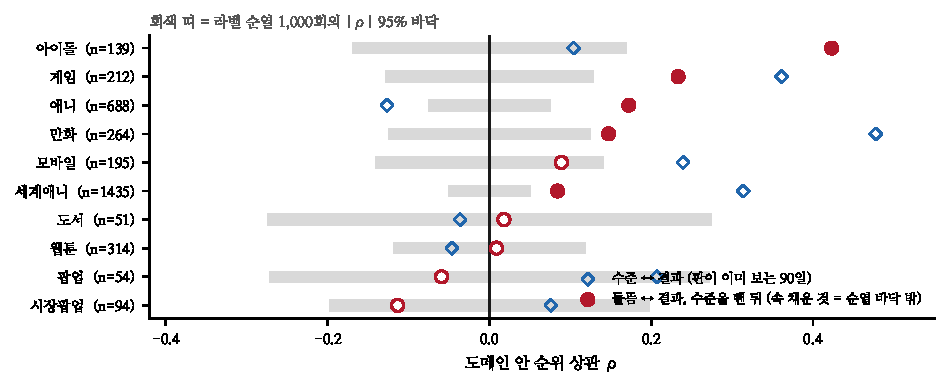
\includegraphics[width=\textwidth]{figs/domains.pdf}
\caption{도메인 안 순위 상관. 회색 띠가 라벨 순열 1{,}000회의 $|\rho|$ 95\%
바닥이고, 속을 채운 붉은 점이 그 밖으로 나간 것이다. 파란 마름모는 판이 이미 보는
90일 \texttt{wiki\_level} 이다. \textbf{바닥을 넘은 다섯이 전부 양수이고, 바닥을
넘은 음수는 없다.}}
\label{fig:dom}
\end{figure*}

10도메인 · 개체 3{,}446을 재서 \textbf{다섯}이 바닥을 넘었고 \textbf{그 다섯이
전부 같은 부호}다. 부호가 음인 둘(시장팝업 $-0.1134$, 팝업 $-0.0591$)은 \textbf{둘
다 자기 바닥 안}이다 --- 즉 \textbf{바닥을 넘은 반대 부호는 0}이다.

\claimx{개체 자신의 오랜 기저 대비 최근 90일의 들뜸은, 최근 90일의 절대 수준이
담지 못한 결과 정보를 담는다.}{바닥을 넘은 도메인의 부호가 갈리면(양과 음이
둘 다 바닥 밖) 이 주장은 깨진다. 실측: 바닥 밖 5 --- 양 5 · 음 0.}

두 자리가 특히 무겁다. \textbf{애니}(n$=$688)는 수준$\leftrightarrow$결과가
\textbf{음수}$(-0.1266)$인데 들뜸은 \textbf{양수}$(+0.1723)$다 --- 두 자가 반대
방향을 가리킨다. \textbf{아이돌}(n$=$139)은 수준 $0.104$ 인데 들뜸이
$\mathbf{0.4230}$ 으로 \textbf{네 배}다. 들뜸이 수준의 단조 변환이었다면 이런 일은
못 생긴다.

\paragraph{들뜸이 그냥 「문서가 새것이다」 아닌가.} 긴 띠의 조회수가 0에 가까우면
들뜸이 커지고, 그것은 \textbf{문서 나이}의 함수다. 그래서 나이(시작일 이전에
조회수 $>0$ 인 날의 수)를 \textbf{하나 더 뺀} 판을 곁에 냈다\footnote{이 검사는
사전등록에 없다. \textbf{사후}다. §4의 자는 바꾸지 않았고 곁에 놓았다.}. 바닥을
넘은 도메인은 \textbf{여전히 다섯이고 여전히 전부 양수}다(아이돌 $0.3184$, 게임
$0.2331$, 만화 $0.1516$, 애니 $0.1459$, 세계애니 $0.0747$). 그리고
「들뜸$\leftrightarrow$나이」의 부호가 도메인마다 \textbf{갈린다}(만화 $+0.49$,
아이돌 $+0.39$ 대 도서 $-0.46$, 세계애니 $-0.37$) --- \textbf{들뜸은 나이의 단조
함수가 아니다.}

\paragraph{증거력의 한계를 먼저 적는다.} ① 이것은 \textbf{연관}이지 예측 성능이
아니다 --- 유보로 안 갈랐다. ② 뺀 것은 \texttt{wiki\_level}(과 사후로 나이)이고
판의 나머지 34열은 안 뺐다. ③ \textbf{영화}(n$=$0)와 \textbf{펀딩}(n$=$2)은 못
쟀다 --- 「효과가 없다」가 아니라 \textbf{「이 원천이 안 덮는다」}이다.

\section{판은 이 자를 못 넘었다 --- 그리고 그것을 미리 적었다}

같은 열을 판에 넣어 씨앗 0$\sim$11로 24주행 했다. \textbf{판은 문턱을 못 넘었다.}
중요한 것은 \textbf{그것이 사전등록의 예측 P2였다}는 점이다.

부착이 $812/3{,}775 = 21.51\%$ 다. 열을 하나 더하면 문턱은 $0.00353$ 이 아니라
$0.01055$ 이고, 판 전체에서 그만큼을 내려면 \textbf{부착된 21.51\% 안에서}
$\Delta\rho \approx 0.049$ 가 필요하다 --- 판 $\rho$ 의 전 역사에서 열 하나가 그
크기를 움직인 전례가 없다. \textbf{그러므로 이 측정이 낼 수 있었던 답은 처음부터
하나뿐이었고, 우리는 그것을 측정 전에 적었다.}

\begin{figure}[t]
\centering

\includegraphics[width=\columnwidth]{figs/board.pdf}
\caption{판 $\rho$ 의 변화와 열 1개 증가 문턱. 막대가 관측, 점선이 문턱이다.}
\label{fig:board}
\end{figure}

\claimx{이 표본에서 판 $\rho$ 는 이 열을 판정할 검출력이 없다. 「못 넘었다」가
아니라 「이 자를 못 넘었다」다.}{부착률을 올리거나(현재 21.51\%) 부착
부분모집단에서 $\Delta\rho \ge 0.049$ 를 보이면 판이 판정할 자격을 얻는다.}

\section{자를 걸었더니 자가 떨어졌다}

도메인 자는 지금까지 한 검사의 \emph{절 회계} 안에만 있었다. 이 노트가 그것을
\textbf{게이트로 꺼냈다}. 걸자마자 \textbf{붉게 떨어졌다} --- 판의 12도메인 중
\textbf{영화}가 이 원천에 한 개체도 없다($\Delta = -1$). 도메인 $\Delta$ 가 네
사이클 연속 0 이었던 것은 자가 안 움직였기 때문이 아니라 \textbf{아무도 자를 실제
원천에 안 걸었기} 때문이었고, 걸자마자 이유가 구체적으로 나왔다 ---
\texttt{ingest/wikidaily941.py} 의 접두 표에 \texttt{KOBIS} 가 \textbf{없다}.
유보 406행이 그 밖에 있다.

\section{그리고 이 노트의 자가 이 노트를 못 갈랐다}

같은 사이클에 상시 조항 하나를 고쳤다 --- \emph{「「모른다」가 분모의 절반을 넘으면
그 자는 그 사이클을 판정할 자격이 없다」}. 그리고 그 조항이 \textbf{같은 사이클에
자기 저자를 물었다}. 항진명제 자를 이 노트의 러너에 돌리니 항진명제는 \textbf{0}
인데 \textbf{14자리 중 13이 「모른다」}였다. 이유는 구조적이다 --- 그 자의 생성기는
모듈 소스에서 열쇠와 문자열을 거두는데, 이 노트의 \texttt{통과} 자리는 numpy
배열과 판 \texttt{Data} 객체를 먹는다. \textbf{생성기가 그런 입력을 원리상 못
만든다.} 그러므로 이 절의 헤드라인은 「항진명제 0」이 아니라 \textbf{「자가 13을 못
갈랐다」}이고, 그것은 \textbf{초록이 아니라 빚}이다.

\end{document}
